%%%%%%%%%%%%%%%%%%%%%%%%%%%%%%%%%%%%%%%%%%%%%%%%%%%%%%%%%%%%%%%%%%%%%%%%%%
%
% Copyright (c) 2012 Jorge Nunes, All Rights Reserved.
%
%%%%%%%%%%%%%%%%%%%%%%%%%%%%%%%%%%%%%%%%%%%%%%%%%%%%%%%%%%%%%%%%%%%%%%%%%%

\documentclass[11pt]{article}

\usepackage[portuges]{babel}
\usepackage[utf8]{inputenc} 
\usepackage{a4}
\usepackage{amsfonts}
\usepackage{float}
\usepackage{graphicx}
\usepackage{subfigure}
\usepackage[colorlinks=true]{hyperref}

\usepackage{parskip}





\title{Cubos Desdobrados}
\author{Jorge Nunes ({\tt\href{mailto:jorgefranconunes@gmail.com}{jorgefranconunes@gmail.com}})}
\date{Dezembro 2007}





\begin{document}


\maketitle

\begin{abstract}
\noindent Neste artigo iremos falar de forma muito introdutória sobre
poliominós e como se relacionam com dobragens de cubos.
\end{abstract}





\section{Introdução}

Poliominós são figuras geométricas compostas por quadrados. Cada
quadrado é adjacente a um ou mais quadrados pelos lados. O número de
quadrados que formam o poliominó corresponde ao seu grau. O jogo
Tetris faz uso de poliominós. A imagem em baixo mostra o estado do
jogo num instante arbitrário. As peças do jogo são poliominós de grau
quatro, ou seja, cada peça é composta por quatro quadrados.

\begin{figure}[H]
  \centering
  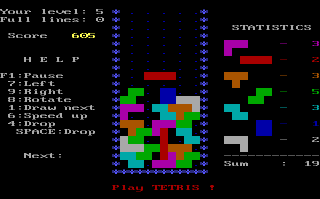
\includegraphics[width=0.66\textwidth]{../images/tetris.png}
  \caption{O jogo Tetris.}
\end{figure}


Note-se que entre os poliominós do Tetris existem dois pares em que as
figuras podem ser obtidas uma da outra através de uma reflexão. As
peças B, C e as peças D, E podem ser obtidas uma da outra através de
uma reflexão.

\begin{figure}[H]
  \centering
  
\includegraphics[width=0.66\textwidth]{../images/poliominos-tetris.pdf}
  \caption{Os poliominós de grau quatro que correspondem às peças do jogo
    Tetris.}
\end{figure}


Existem duas classes comuns de classificação de poliominós. Poliominós
de lado único e poliominós de forma livre.

\begin{itemize}

\item Poliominós do lado único --- São poliominós que não podem ser
  obtidos uns dos outros por qualquer composição de rotações. As
  figuras do Tetris formam o conjunto dos poliominós de grau quatro de
  lado único.

\item Poliominós de forma livre --- São poliominós que não podem ser
  obtidos uns dos outros por qualquer composição de rotações e
  reflexões.

\end{itemize}





\section{Geração de Poliominós}

A geração de poliominós é extremamente simples. Dados os poliominós de
grau $n-1$ podem obter-se todos os poliominós de grau $n$. O procedimento
para a obtenção de todos os poliominós de grau $n$ é pois recursivo. O
processo tem início com o único poliominó de grau 2, formado por dois
quadrados.

O procedimento para obtenção dos poliominós de grau $n$ envolve tratar
cada um dos poliominós de grau $n-1$ da forma descrita em seguida.

Dado um poliominó de grau $n-1$ são gerados poliominós de grau $n$
adicionando à figura um novo quadrado em cada uma das posições
possíveis. Na imagem em baixo está ilustrado este processamento. A
figura cinzenta representa o poliominó original. O quadrado vermelho
representa o quadrado que é adicionado à figura original em cada uma
das posições possíveis.

\begin{figure}[H]
  \centering
  
\includegraphics[width=0.66\textwidth]{../images/poliominos-step.pdf}
  \caption{Geração de poliominós de grau $n$ a partir de um poliominó
    de grau $n-1$.}
\end{figure}


Para cada um dos poliominós assim obtidos determina-se se devem ser
adicionados à lista de poliominós de grau $n$ encontrados até ao
momento. Para tal verifica-se se o poliominó pode ser obtido de um dos
poliominós já encontrados. Se estamos a gerar poliominós de lado único
verifica-se se pode ser obtido de rotações. Se estamos a gerar
poliominós de forma livre verifica-se se pode ser obtido por uma
composição de rotações e reflexão.





\section{Exemplos de Poliominós}

Vamos de seguida apresentar os conjuntos de poliominós de forma livre
até ao grau 7.


\subsection{Monominós}

Poliominós de grau 1 (monominós) são compostos por um único
quadrado. Destes, obviamente, existe apenas um.


\subsection{Dominós}

Existe também apenas um único poliominó de grau 2, composto por dois
quadrados.


\subsection{Triminós}

Poliominós de grau 3 são também designados por triminós, dos quais
existem apenas 2.

\begin{figure}[H]
\centering
  
\includegraphics[width=0.15\textwidth]{../images/poliominos-3-free.pdf}
\caption{Triminós.}
\end{figure}


\subsection{Tetrominós}

Os poliominós de grau 4 são as peças do jogo Tetris. Existem 5 na
forma livre, visíveis na figura seguinte.

\begin{figure}[H]
\centering
  
\includegraphics[width=0.4\textwidth]{../images/poliominos-4-free.pdf}
\caption{Tetrominós.}
\end{figure}


\subsection{Pentominós}

Outra designação dos poliominós de grau 5. Existem 12 deles.

\begin{figure}[H]
\centering
  
\includegraphics[width=\textwidth]{../images/poliominos-5-free.pdf}
\caption{Pentominós}
\end{figure}


\subsection{Hexominós}

Existem 35 poliominós de grau 6 distintos.

\begin{figure}[H]
\centering
  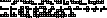
\includegraphics[width=\textwidth]{../images/poliominos-6-free.pdf}
\caption{Hexominós.}
\end{figure}


\subsection{Heptominós}

Existem 108 poliominós de grau 7.

\begin{figure}[H]
\centering
  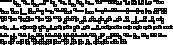
\includegraphics[width=\textwidth]{../images/poliominos-7-free.pdf}
\caption{Heptominós.}
\end{figure}





\section{Dobragens de Cubos}

Alguns dos poliominós de grau 6 são dobragens de cubo. Por dobragem de
cubo entendemos uma figura que por meio de dobragens apropriadas possa
transformar-se num cubo. Cada dobragem individual tem sempre como eixo
um lado de um dos quadrados que formam o hexaminó. Não é permitido
"rasgar" a figura em qualquer um dos passos das dobragens.

As imagens seguintes ilustram um exemplo da dobragem de um cubo a
partir de um hexominó. Cada imagem corresponde a um passo da sequência
de dobragens desde a figura plana inicial (o hexominó) até chegar ao
cubo.

\begin{figure}[H]
  \centering

  \subfigure[]{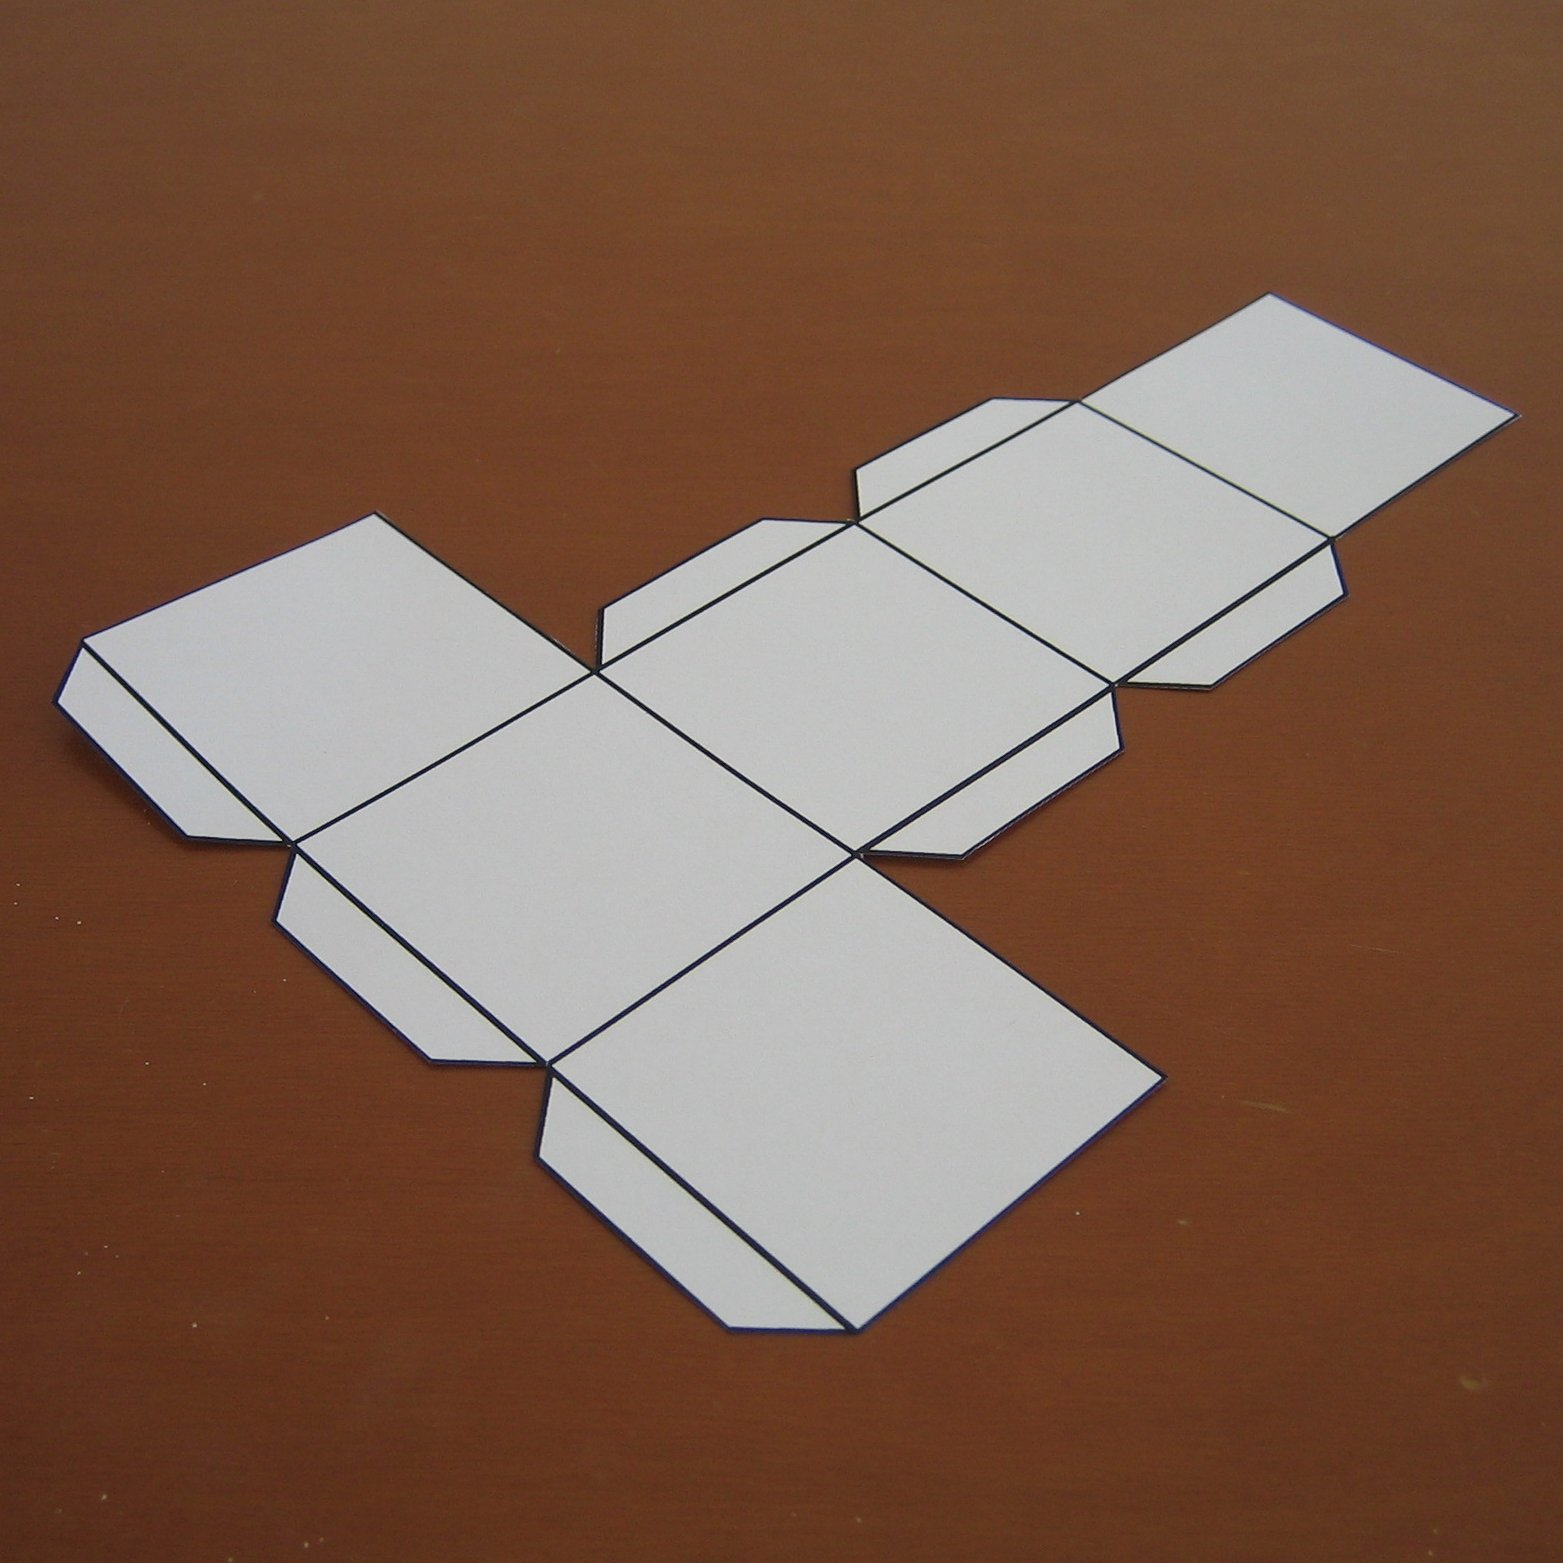
\includegraphics[width=0.3\textwidth]{../images/Step-01.jpg}}
  \subfigure[]{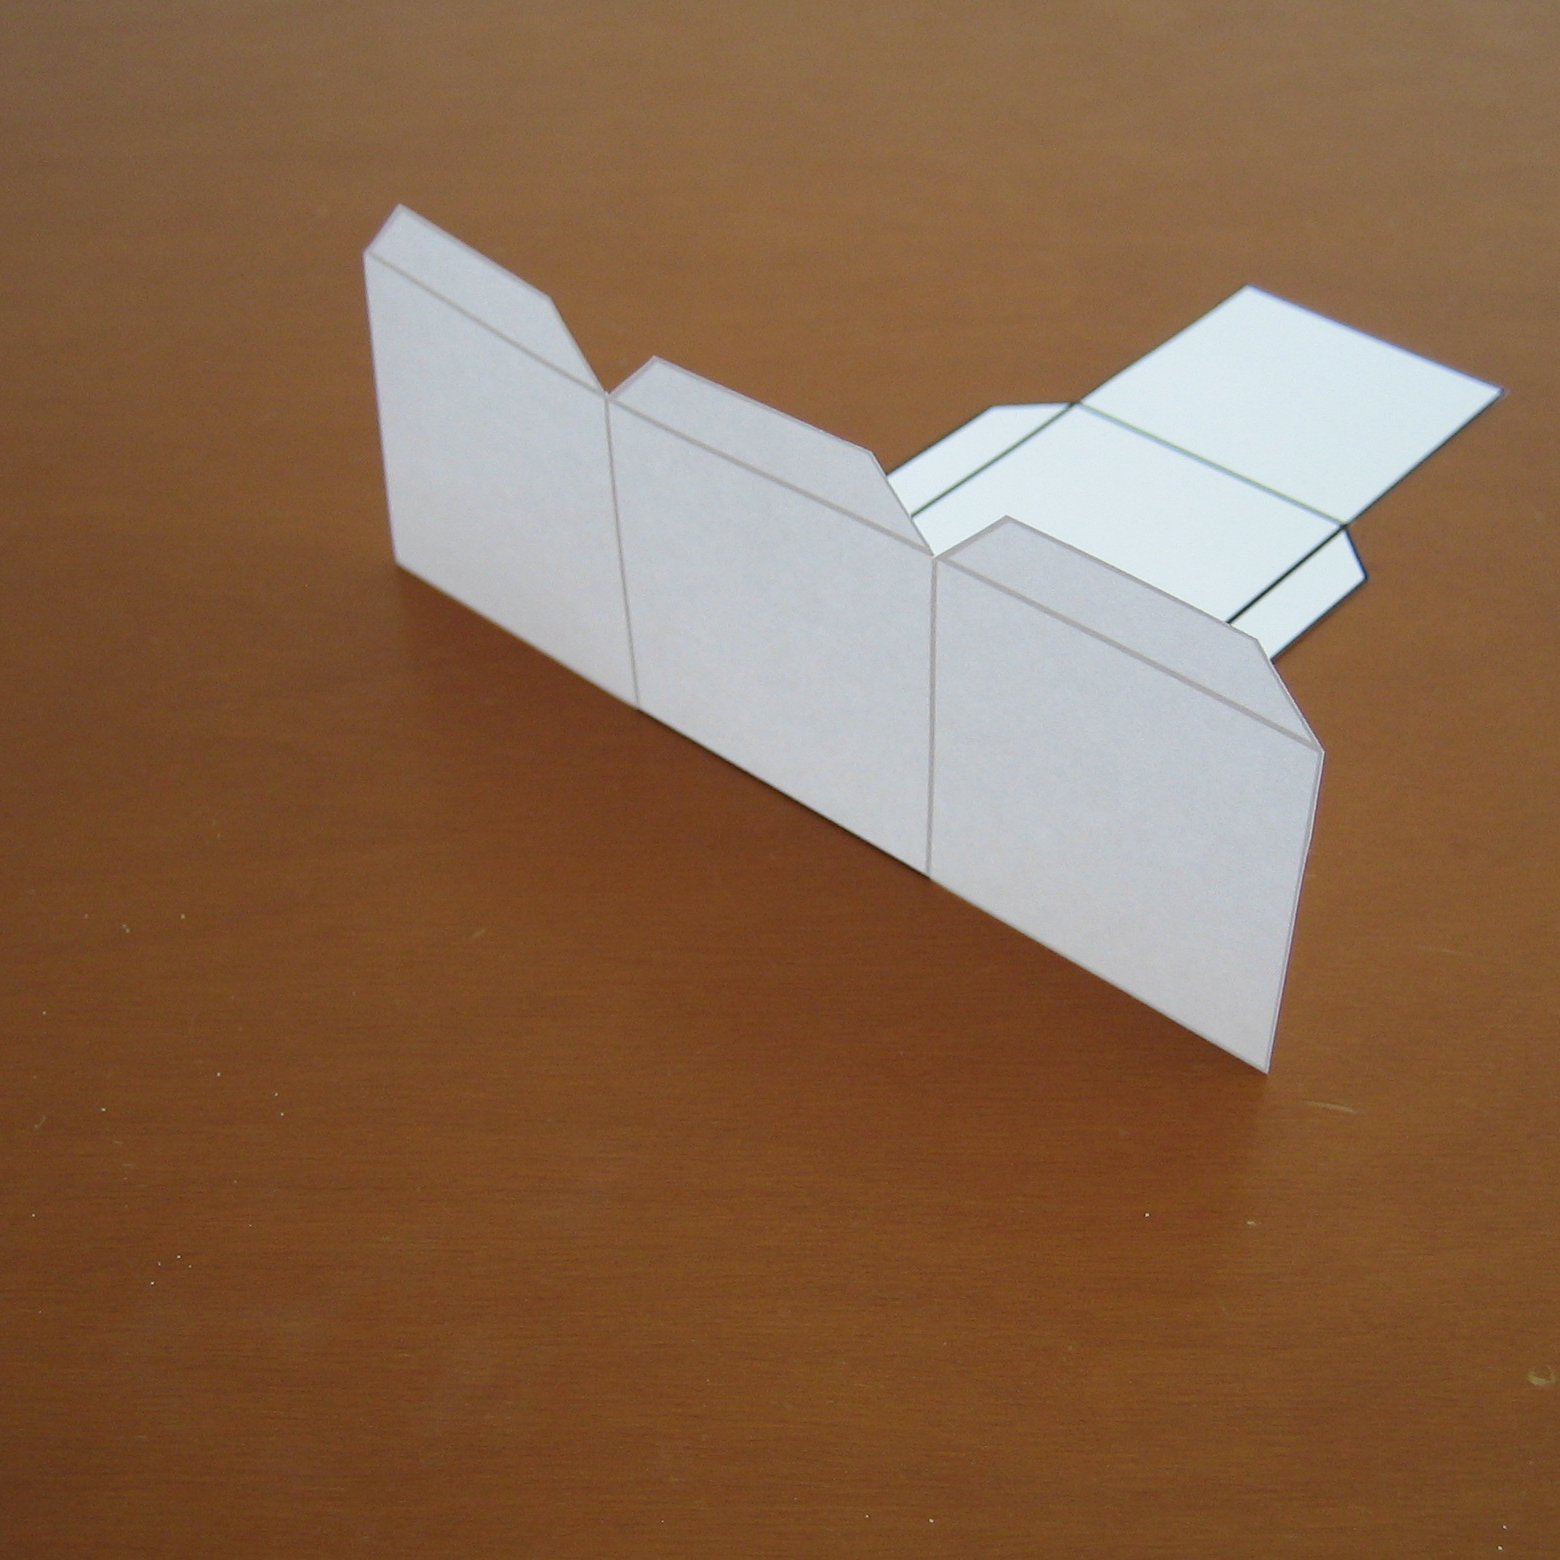
\includegraphics[width=0.3\textwidth]{../images/Step-02.jpg}}
  \subfigure[]{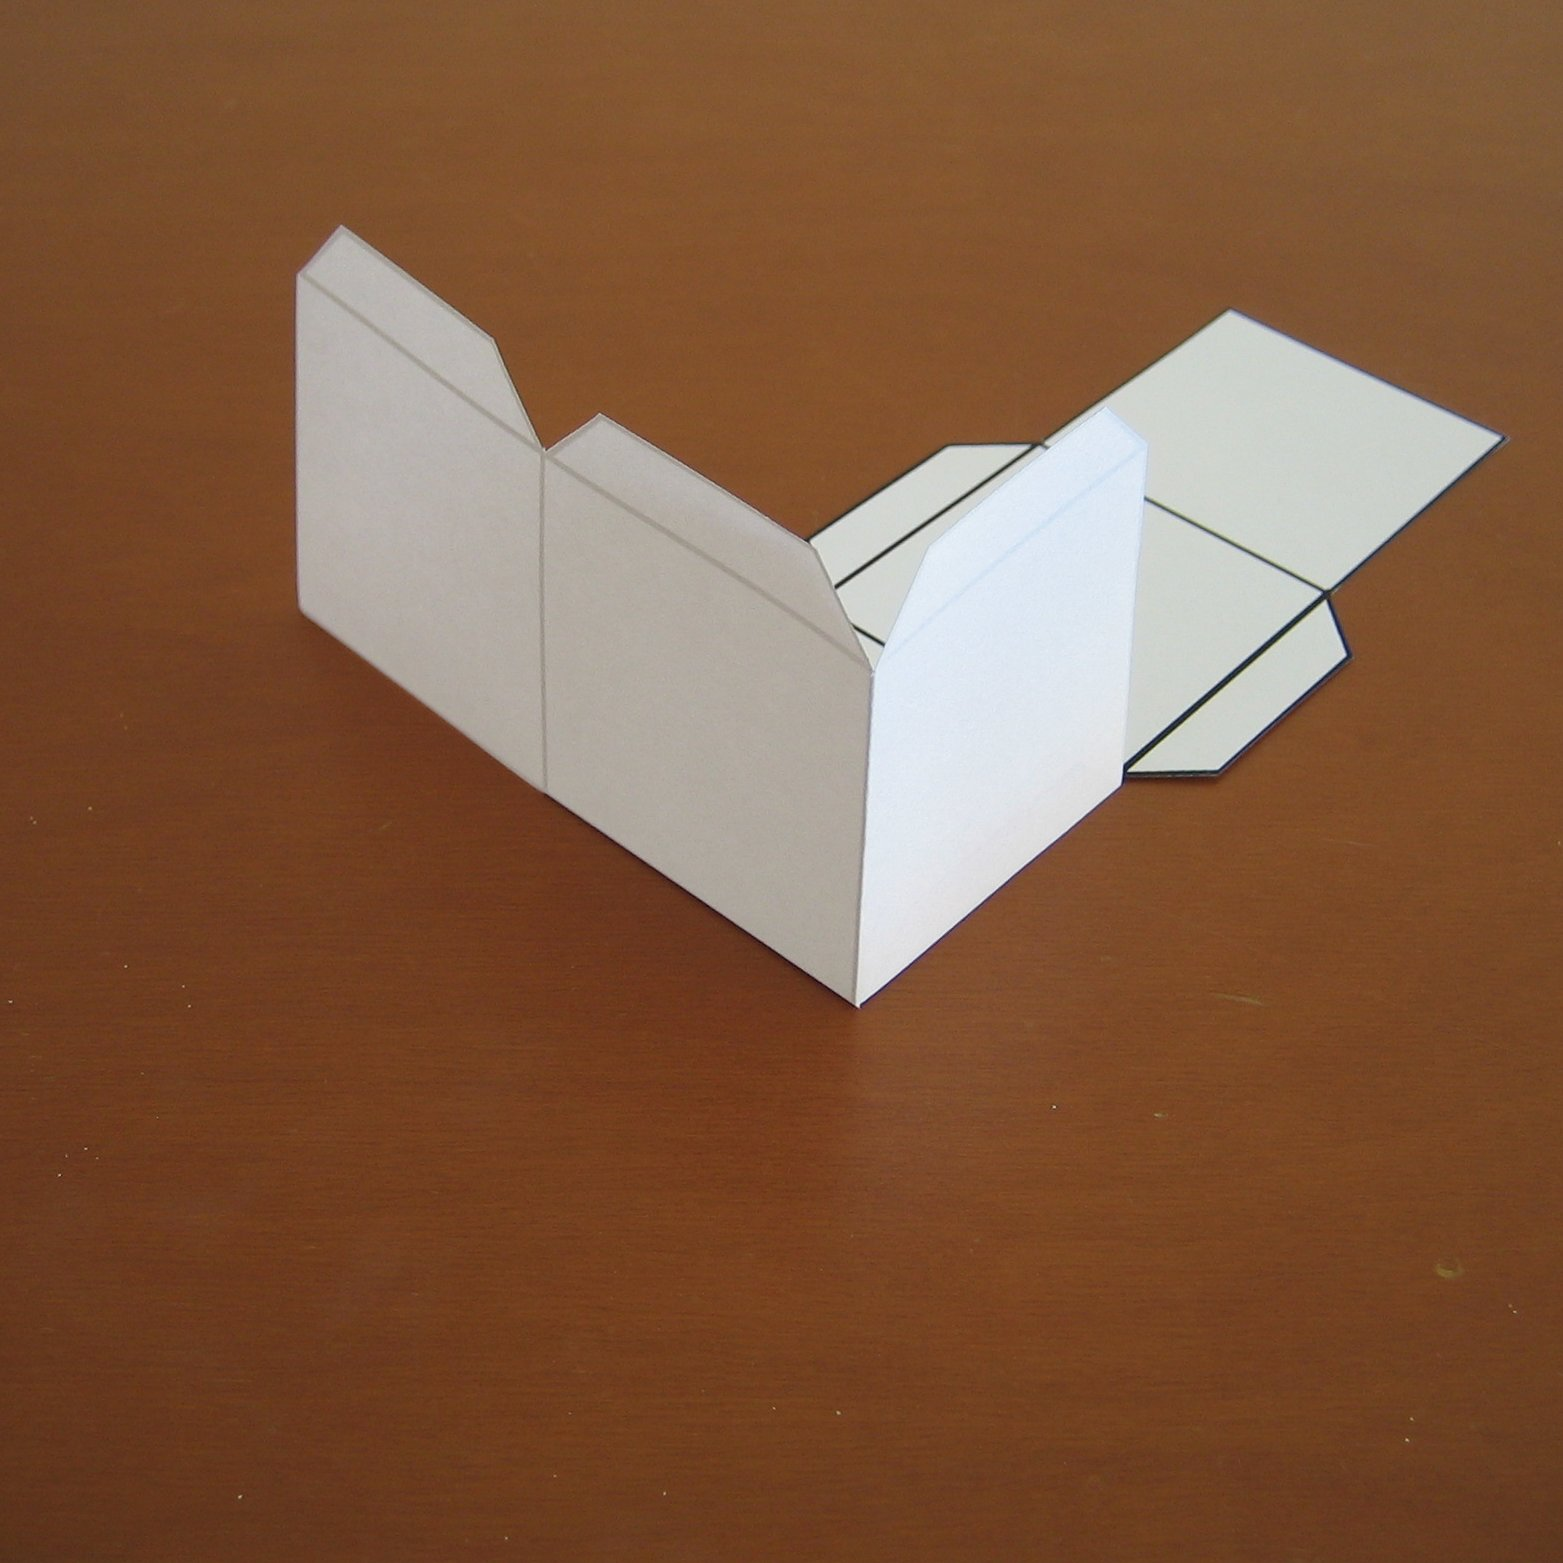
\includegraphics[width=0.3\textwidth]{../images/Step-03.jpg}}

  \subfigure[]{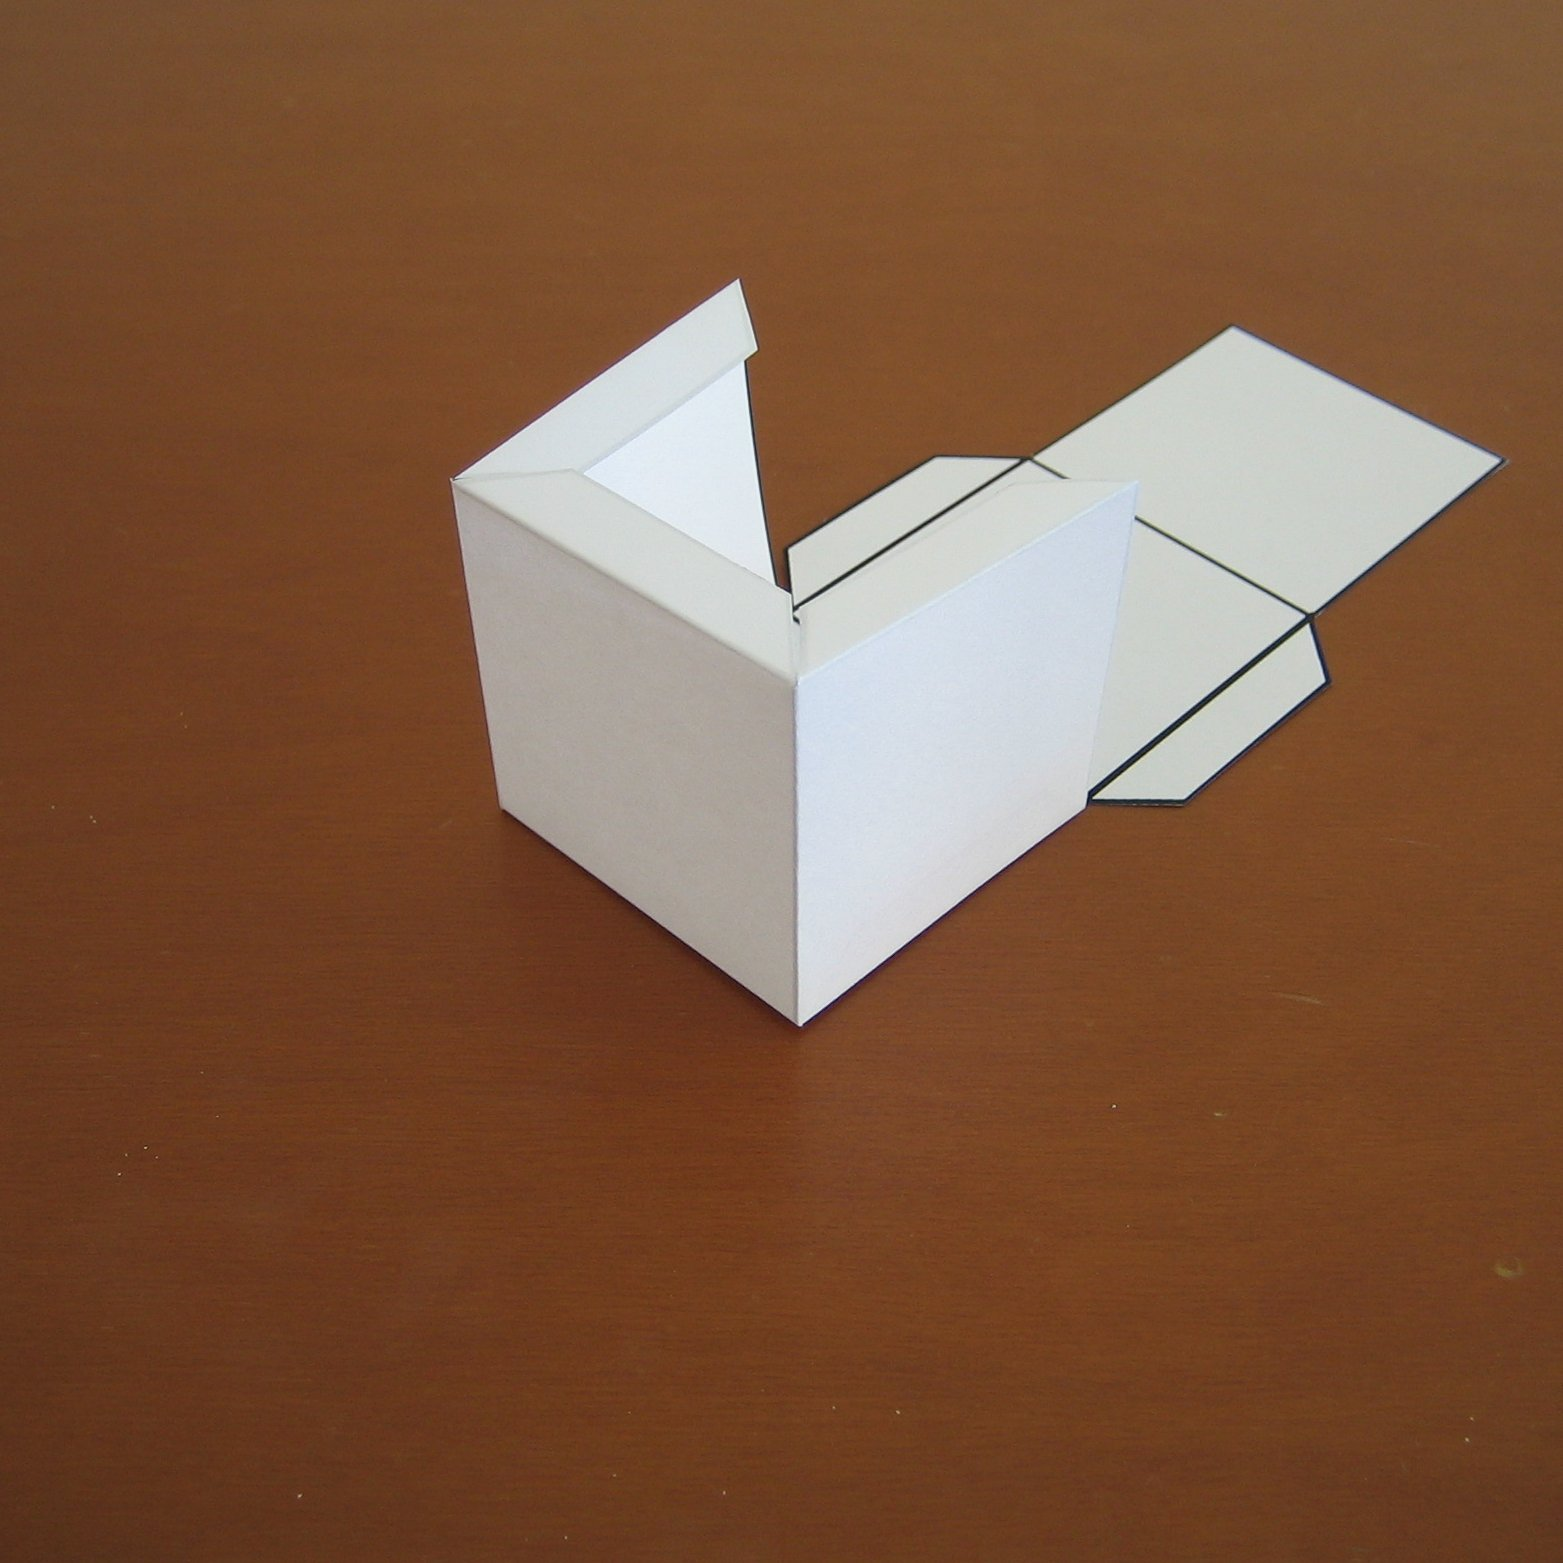
\includegraphics[width=0.3\textwidth]{../images/Step-04.jpg}}
  \subfigure[]{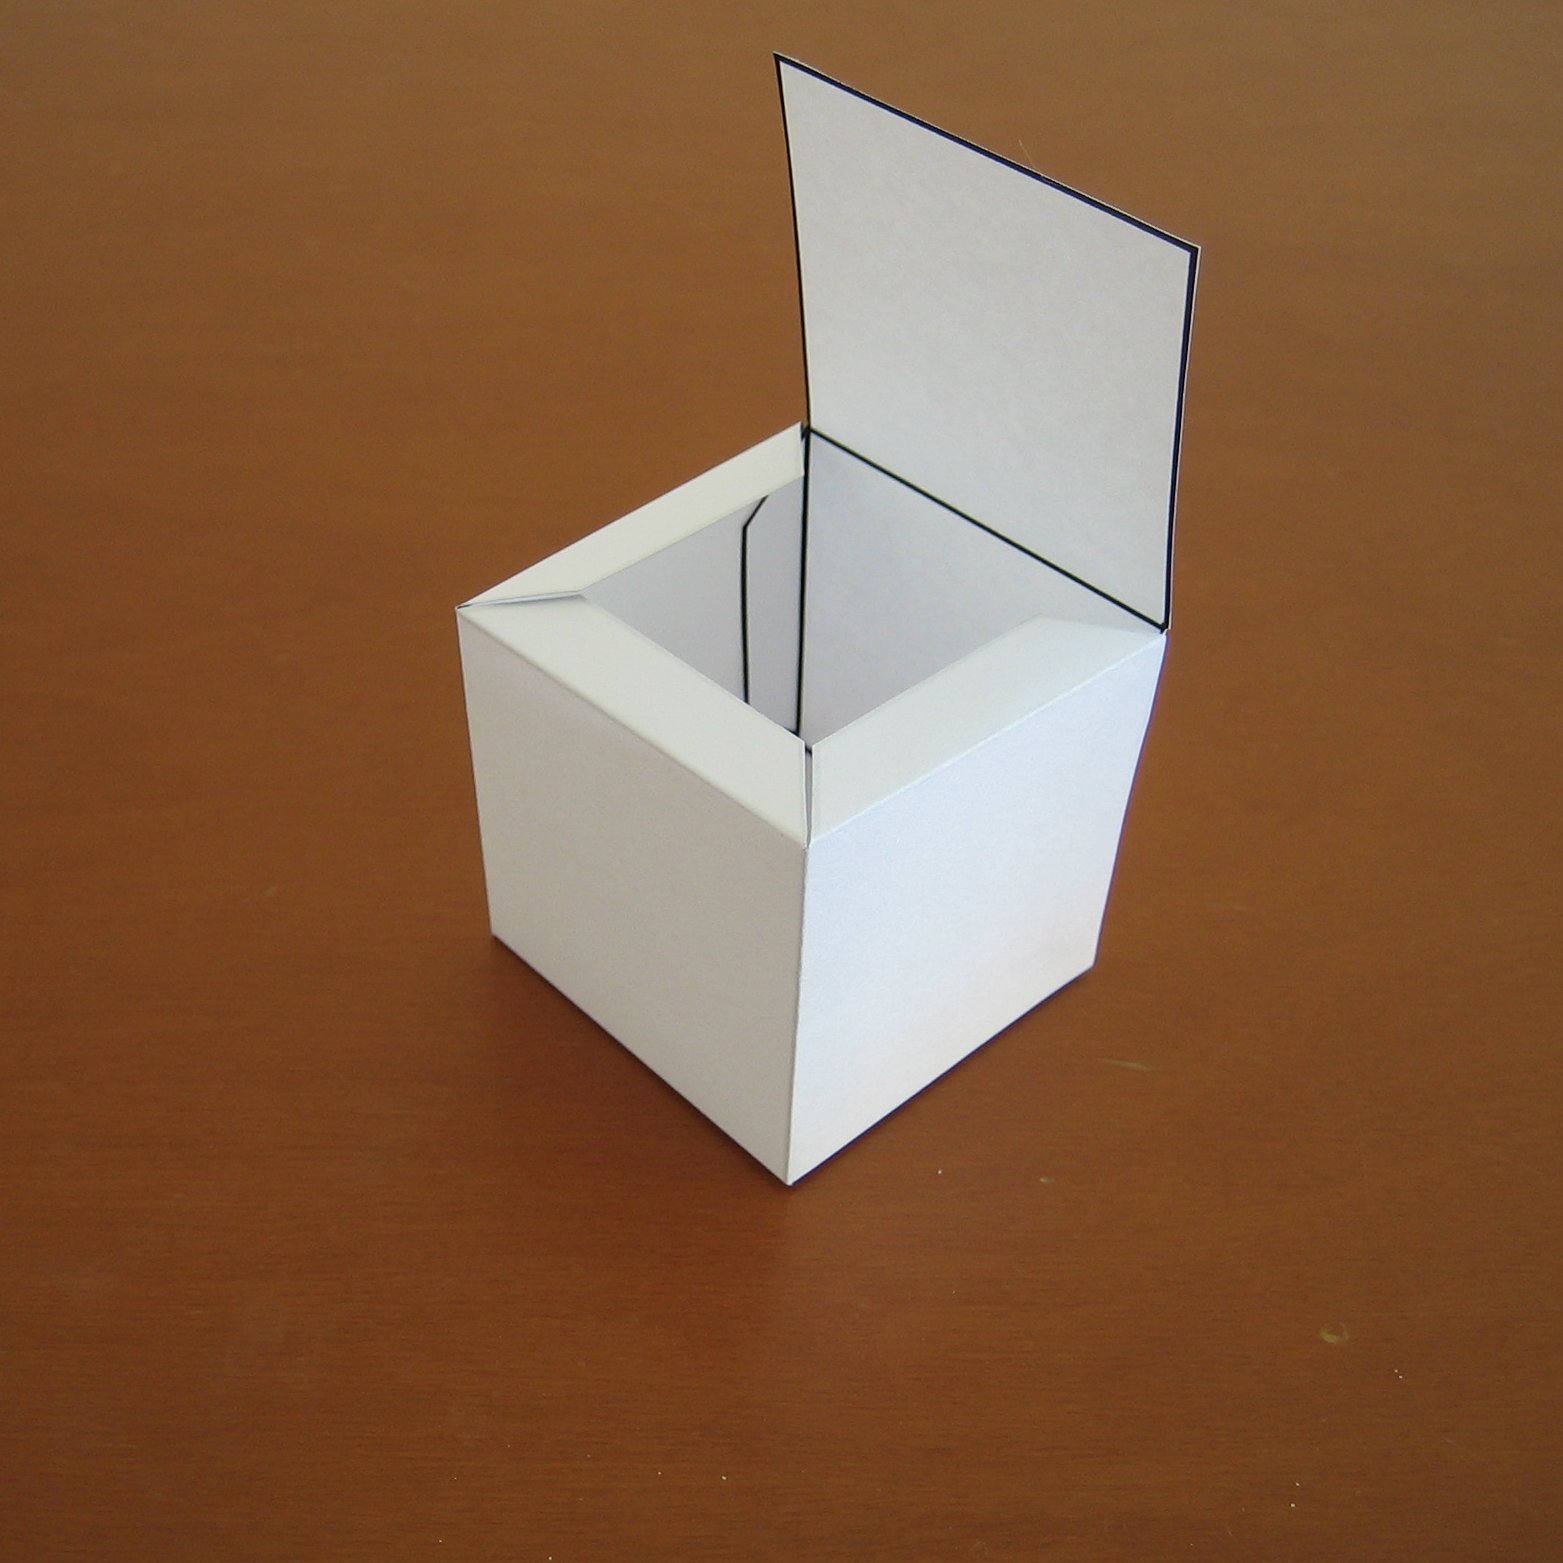
\includegraphics[width=0.3\textwidth]{../images/Step-05.jpg}}
  \subfigure[]{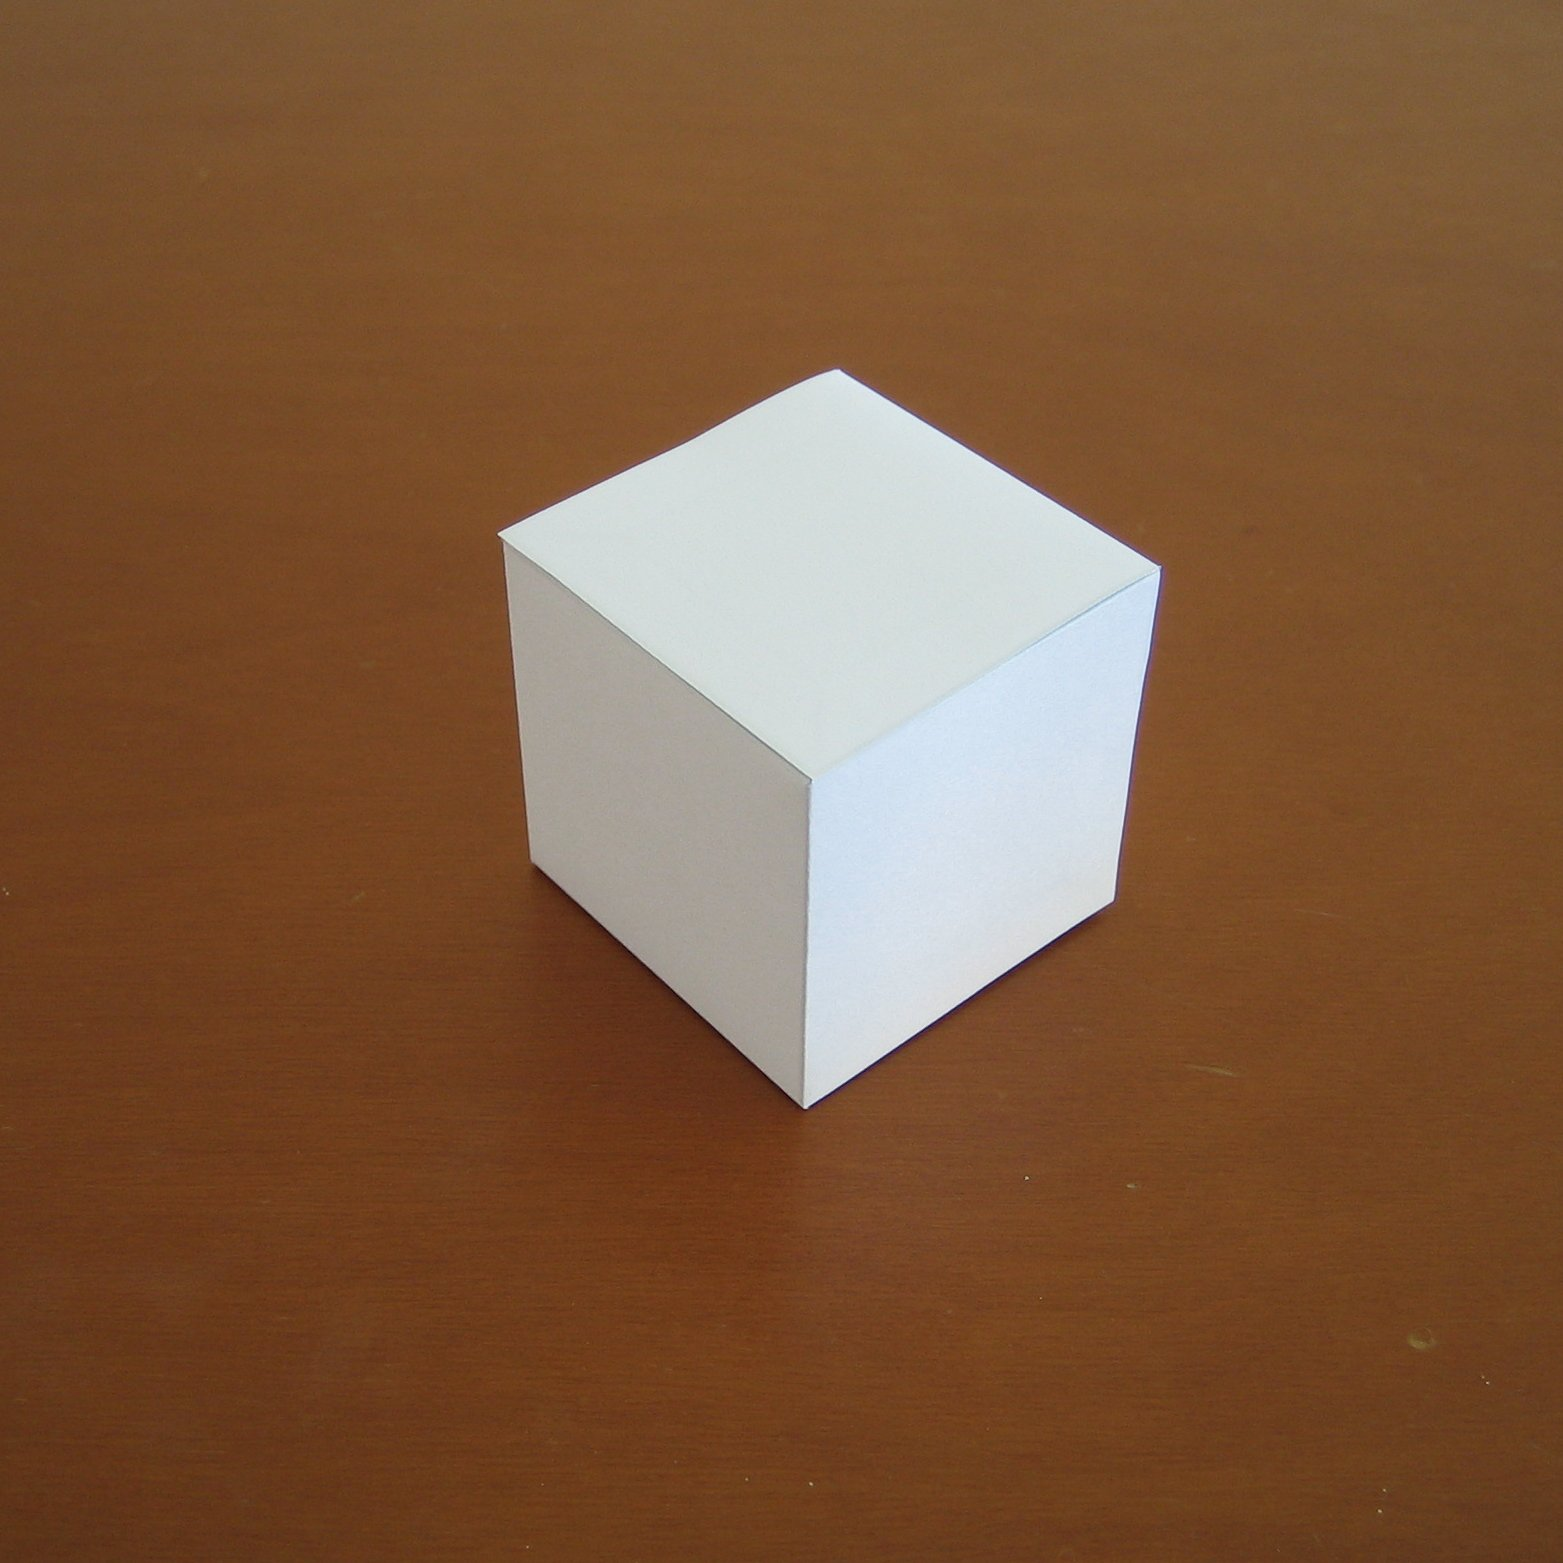
\includegraphics[width=0.3\textwidth]{../images/Step-06.jpg}}

  \caption{Os passos da dobragem de um cubo a partir de um hexaminó.}
\end{figure}


Todos os poliominós de grau 6 de forma livre que correspondem a
dobragens de um cubo estão indicados na figura em baixo.

\begin{figure}[H]
\centering
  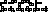
\includegraphics[width=0.5\textwidth]{../images/poliominos-cubo.pdf}
\caption{Hexominós que correspondem a dobragens de um cubo.}
\end{figure}


Estes hexominós foram encontrados inspeccionando visualmente cada um
dos 35 hexominós de lado único. A questão que vamos deixar no ar é se
existirá algum algoritmo que permita classificar de forma simples um
dado hexominó como sendo, ou não, uma dobragem de cubo. Ou, de forma
quase equivalente, qual o algoritmo que permite gerar todos os
hexominós que são dobragens de um cubo. Esperamos ter resultados para
um artigo futuro.





\section*{Referências}

\begin{itemize}

\item \href{http://en.wikipedia.org/wiki/Polyomino}{Wikipedia:Polyomino}.

\item
  \href{http://www.mat.uc.pt/~jaimecs/nonius/nonius16_1.html}{Nonius
    nº 16 - Recensões Críticas de Software}.

\end{itemize}





\section*{Cólofon}

As imagens PNG usadas neste artigo com figuras de poliominós foram
geradas com \href{http://www.inkscape.org/}{Inkscape} a partir de
ficheiros SVG.

Os ficheiros SVG com figuras de poliominós foram gerados a partir de
um programa para geração de poliominós escrito na linguagem de
scripting \href{http://www.pdmfc.com/tea-site/info/index.html}{Tea}.





\end{document}

